\documentclass[12pt,a4paper]{article}
\usepackage{lmodern}

\usepackage{placeins}
\usepackage{booktabs}
\usepackage{amssymb,amsmath}
\usepackage{ifxetex,ifluatex}
\usepackage{fixltx2e} % provides \textsubscript
\ifnum 0\ifxetex 1\fi\ifluatex 1\fi=0 % if pdftex
  \usepackage[T1]{fontenc}
  \usepackage[utf8]{inputenc}
\else % if luatex or xelatex
  \ifxetex
    \usepackage{mathspec}
    \usepackage{xltxtra,xunicode}
  \else
    \usepackage{fontspec}
  \fi
  \defaultfontfeatures{Mapping=tex-text,Scale=MatchLowercase}
  \newcommand{\euro}{€}
\fi
% use upquote if available, for straight quotes in verbatim environments
\IfFileExists{upquote.sty}{\usepackage{upquote}}{}
% use microtype if available
\IfFileExists{microtype.sty}{%
\usepackage{microtype}
\UseMicrotypeSet[protrusion]{basicmath} % disable protrusion for tt fonts
}{}
\usepackage[lmargin = 3 cm,rmargin = 2.5cm,tmargin=2.5cm,bmargin=2.5cm]{geometry}

% Figure Placement:
\usepackage{float}
\let\origfigure\figure
\let\endorigfigure\endfigure
\renewenvironment{figure}[1][2] {
    \expandafter\origfigure\expandafter[H]
} {
    \endorigfigure
}

%% citation setup
\usepackage{csquotes}

\usepackage[backend=biber, maxbibnames = 99, style = apa]{biblatex}
\setlength\bibitemsep{1.5\itemsep}
\addbibresource{R_packages.bib}
\bibliography{references.bib}
\usepackage{graphicx}
\makeatletter
\def\maxwidth{\ifdim\Gin@nat@width>\linewidth\linewidth\else\Gin@nat@width\fi}
\def\maxheight{\ifdim\Gin@nat@height>\textheight\textheight\else\Gin@nat@height\fi}
\makeatother
% Scale images if necessary, so that they will not overflow the page
% margins by default, and it is still possible to overwrite the defaults
% using explicit options in \includegraphics[width, height, ...]{}
\setkeys{Gin}{width=\maxwidth,height=\maxheight,keepaspectratio}
\ifxetex
  \usepackage[setpagesize=false, % page size defined by xetex
              unicode=false, % unicode breaks when used with xetex
              xetex]{hyperref}
\else
  \usepackage[unicode=true, linktocpage = TRUE]{hyperref}
\fi
\hypersetup{breaklinks=true,
            bookmarks=true,
            pdfauthor={Jens Klenke, Nils Paffen},
            pdftitle={The Irish Electricity Market},
            colorlinks=true,
            citecolor=blue,
            urlcolor=blue,
            linkcolor=magenta,
            pdfborder={0 0 0}}
\urlstyle{same}  % don't use monospace font for urls
\setlength{\parindent}{0pt}
\setlength{\parskip}{6pt plus 2pt minus 1pt}
\setlength{\emergencystretch}{3em}  % prevent overfull lines
\setcounter{secnumdepth}{5}

%%% Use protect on footnotes to avoid problems with footnotes in titles
\let\rmarkdownfootnote\footnote%
\def\footnote{\protect\rmarkdownfootnote}

%%% Change title format to be more compact
\usepackage{titling}

% Create subtitle command for use in maketitle
\newcommand{\subtitle}[1]{
  \posttitle{
    \begin{center}\large#1\end{center}
    }
}

\setlength{\droptitle}{-2em}
  \title{The Irish Electricity Market}
  \pretitle{\vspace{\droptitle}\centering\huge}
  \posttitle{\par}
\subtitle{A forcestaing Study for the half-hourly Day-Ahead Prices}
  \author{Jens Klenke, Nils Paffen}
  \preauthor{\centering\large\emph}
  \postauthor{\par}
  \predate{\centering\large\emph}
  \postdate{\par}
  \date{today}


%% linespread settings

\usepackage{setspace}

\onehalfspacing

% Language Setup

\usepackage{ifthen}
\usepackage{iflang}
\usepackage[super]{nth}
\usepackage[ngerman, english]{babel}

%Acronyms
\usepackage[printonlyused, withpage, nohyperlinks]{acronym}
\usepackage{changepage}

% Multicols for the Title page
\usepackage{multicol}

\begin{document}

\selectlanguage{english}


%\maketitle

\begin{titlepage}
  \noindent\begin{minipage}{0.6\textwidth}
	  \IfLanguageName{english}{University of Duisburg-Essen}{Universität Duisburg-Essen}\\
	  \IfLanguageName{english}{Faculty of Business Administration and Economics}{Fakultät für Wirtschaftswissensschaften}\\
	  \IfLanguageName{english}{Chair of Economeics}{Lehrstuhl für Wirtschaftswissenschaften}\\
  \end{minipage}
	\begin{minipage}{0.4\textwidth}
	  \begin{flushright}
  	  \vspace{-0.5cm}
      \IfLanguageName{english}{\includegraphics*[width=5cm]{Includes/duelogo_en.png}}{\includegraphics*[width=5cm]{Includes/duelogo_de.png}}
	  \end{flushright}
	\end{minipage}
  \\
  \vspace{0.5cm}
  \begin{center}
  \huge{The Irish Electricity Market}\\
  \vspace{.25cm}
  \Large{A forcestaing Study for the half-hourly Day-Ahead Prices}\\
  \vspace{0.5cm}
  \large{Seminar Paper}\\
  \vspace{0.5cm}
  \large{  \IfLanguageName{english}{Submitted to the Faculty of \\ Economics  \\at the \\University of Duisburg-Essen}{Vorgelegt der \\Fakultät für Wirtschaftswissenschaften der \\ Universität Duisburg-Essen}\\}
  \vspace{0.75cm}
  \large{\IfLanguageName{english}{from:}{von:}}\\
  \vspace{0.5cm}
  Jens Klenke, Nils Paffen\\
  \end{center}
  %\vspace{2cm}
  \vfill
  \hrulefill

  \noindent\begin{minipage}[t]{0.3\textwidth}
  \IfLanguageName{english}{Reviewer:}{Erstgutachter:}
  \end{minipage}
  \begin{minipage}[t]{0.7\textwidth}
  \hspace{1cm}Prof.~Dr.~Florian Ziel
  \end{minipage}

  \noindent\begin{minipage}[t]{0.3\textwidth}
  \IfLanguageName{english}{Deadline:}{Abgabefrist:}
  \end{minipage}
  \begin{minipage}[t]{0.7\textwidth}
  \hspace{1cm}Jan.~27th 2020
  \end{minipage}

  \hrulefill

  \begin{multicols}{3}

  Name:

  Matriculation Number:

  E-Mail:

  Study Path:

  Semester:

  Graduation (est.):
 
  \columnbreak

  Jens Klenke

  3071594
  
  jens.klenke@stud.uni-due.de

  M.Sc. Economics

  \nth{5}

  Winter Term 2020
  
  \columnbreak

  Nils Paffen

  30
  
  nils.paffen@stud.uni-due.de

  M.Sc. Economics

  \nth{2}

  Winter Term 2021

	\end{multicols}

\end{titlepage}

\newgeometry{top=2cm, left = 5cm, right = 2.5cm, bottom = 2.5cm}


\pagenumbering{Roman}
{
\hypersetup{linkcolor=black}

\setcounter{tocdepth}{3}
\tableofcontents
}

\newpage
\listoffigures
\addcontentsline{toc}{section}{List of Figures}

%\newpage
\listoftables
\addcontentsline{toc}{section}{List of Tables}

\section*{List of Abbreviations}
\addcontentsline{toc}{section}{List of Abbreviations}

\begin{adjustwidth}{1.5em}{0pt}

\begin{acronym}[dummyyyy]
 \acro{LASSO}{Least Absolute Shrinkage and Selection Operator}
 \acro{pcr}{Principal Components Regression}
 \acro{RMSE}{Root Mean Squared Error}
 \acro{MAE}{Mean Absolute Error}
 \acro{SEM}{Single Electricity Market}
 \acro{I-SEM}{Integrated Single Electricity Market}
 \acro{EU}{European Union}
 \acro{DM}{Diebold-Mariano}


%Falls eine Abkürzung in der Mehrzahl nicht einfach auf "s" endet muss das speziell eingestellt werden.
% \acro{slmtA}{super lange mega tolle Abkürzung} %Einzahl
 %\acroplural{slmtA}[slmtAs]{super lange mega tolle Abkürzungen} %Mehrzahl
 \acro{dummyyyy}{dummyyy}
\end{acronym}

\end{adjustwidth}

\restoregeometry

\newpage
\pagenumbering{arabic}
\hypertarget{introduction}{%
\section{Introduction}\label{introduction}}

In this paper we want to analyse and predict the Day-Ahead prices for
Irleand. On the first of October 2018 Ireland moved from the \ac{SEM}
market to the \ac{I-SEM} market in order to further strengthen its
integration with the \ac{EU}. \autocite{eridgrid_i-sem_2020}

The Day-Ahead price is very important for all market participants to
decide if there should commit to sell or buy at the market. In recent
years, predicting day-ahead prices has become increasingly difficult due
to the larger share of renewable energies and the new resulting pricing
structures. \autocite{ziel_efficient_2015}

First, the Irish Electricity Market is described and the data we have
received about that market is described. Next the benchmark model is
presented and then the advanced models are estimated before a conclusion
is drawn.

\hypertarget{the-irish-electricity-market}{%
\section{The Irish Electricity
Market}\label{the-irish-electricity-market}}

The Irish electricity market was established in 2007 (\ac{SEM}) and has
not been reformed in a wider sense until the \ac{I-SEM} market was
introduced in 2018. In the period(s) leading up to the integrated market
in October 2018, there has been some adjustment and therefore a higher
volatility in the market.

\FloatBarrier
\begin{figure}

{\centering \includegraphics[width=1\linewidth]{C:/Users/Anwender/Documents/GitHub/EEM/04_output/fuel_mix_for_electricity_gen_IRE_2019} 

}

\caption{ \label{fig:energy_mix} Primary fuel mix for electricity generation}\label{fig:fig_energy_mix}
\end{figure}
\FloatBarrier

Figure \ref{fig:energy_mix} shows relatively clearly that Ireland
generates a large part of its primary energy from gas. Furthermore, it
can be seen that the share of renewable energies has increased
relatively strongly. The average growth rate of renewable energy was
10.7 percent between 2015 and 2018. \autocite{dineen_energy_2019}

\hypertarget{data-description}{%
\section{Data Description}\label{data-description}}

\FloatBarrier
\begin{figure}

\includegraphics[width=1\linewidth]{C:/Users/Anwender/Documents/GitHub/EEM/04_output/timeline} \hfill{}

\caption{ \label{fig:timeline} Half-hourly Day-Ahead Prices in Irland}\label{fig:fig_timeline}
\end{figure}
\FloatBarrier

Our Data contained \emph{152} variables from the first of January 2015
till 30 of October 2019. Due to the fact that Ireland has changed the
market from the \ac{SEM} to the \ac{I-SEM} (market integration with the
\ac{EU}) and thus switched from half-hourly products to hourly products,
the trajectory from 25 October 2015 to 28 September 2018 has been
shortened. Therefore, only 1070 full days are left for estimating and
testing, which is about 2.9 years. Due to the change from half-hourly to
hourly products, there is also the problem that either only about 9
tenths of a year are left for testing, with 2 years for estimation, or
only one year for estimation if you want to have more than one year for
testing. \autocite{cashman_i-sem_2019}

\FloatBarrier
\begin{figure}

{\centering 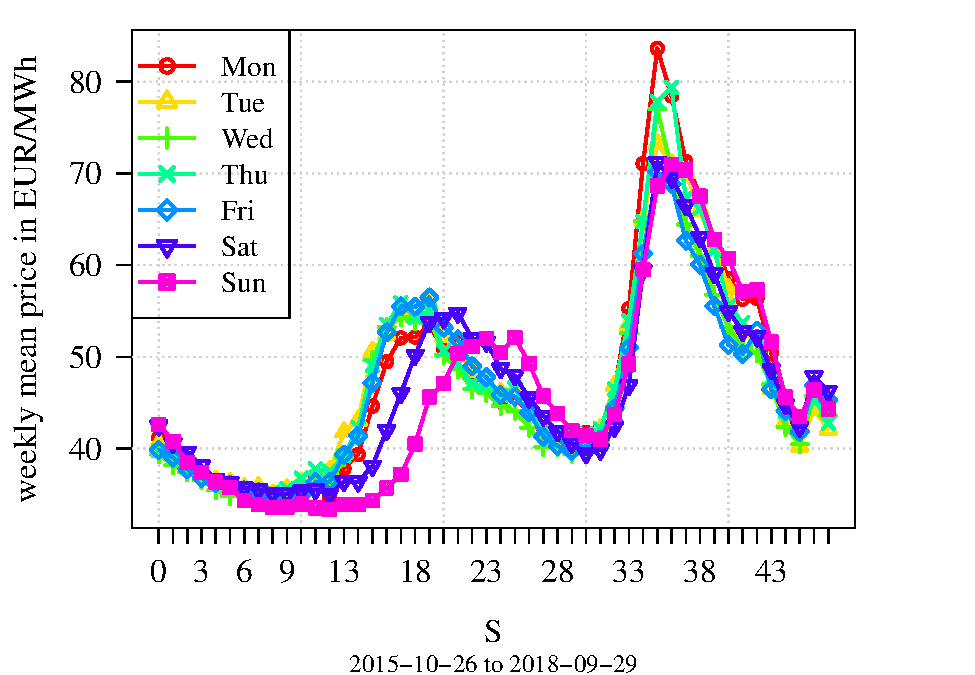
\includegraphics[width=0.45\linewidth]{term_paper_eem_files/figure-latex/unnamed-chunk-2-1} 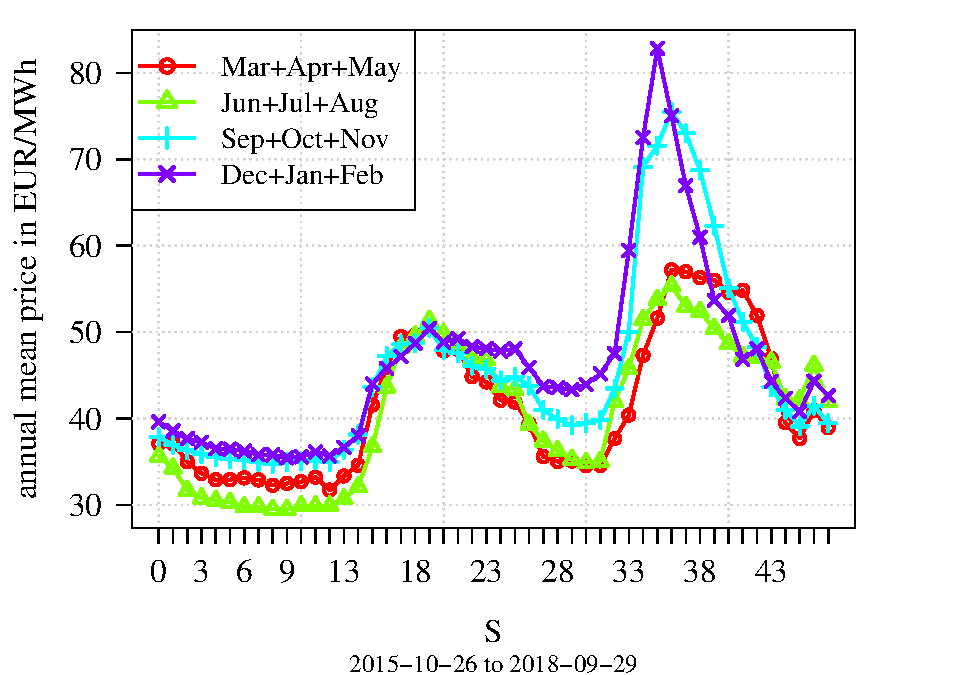
\includegraphics[width=0.45\linewidth]{term_paper_eem_files/figure-latex/unnamed-chunk-2-2} 

}

\caption{ \label{fig:structure} Mean Values Weekdays and quarters of the year  }\label{fig:unnamed-chunk-2}
\end{figure}
\FloatBarrier

Both cases are not optimal, as one can also see in Figure
\ref{fig:timeline}. For the estimation of annual cycles at least 2 years
would be preferable. On the other hand, you actually need at least one
year in the test data set to benefit from the estimates of the annual
components.

Our goal is to predict the price for the next day, so we can only use
data that is already known at the time of the forecast (day-ahead). As
can be seen from Table \ref{tab:data}, there is little data in our data
set for this purpose. For solar and offshore energy there is no data at
all and for onshore energy about half of the data is missing. Only for
the load for the next day we have about 98 percent of the data, which
may be implied in a multivariate model.

\begin{table}[]
\centering
\begin{tabular}{@{}llllll@{}}
\toprule
Date    & Price   & Solar     & Offshore  & Onshore  & Load    \\ \midrule
0,00 \% & 0,18 \% & 100,00 \% & 100,00 \% & 50,74 \% & 2,59 \% \\ \bottomrule
\end{tabular}
\caption{Proportions of NA's in important Day Ahead variables}
\label{tab:data}
\end{table}

\hypertarget{basic-models}{%
\section{Basic Models}\label{basic-models}}

Two relatively simple models are to be estimated as a benchmark for the
models that will follow later.

The first model is the \emph{naive model} which is relatively simple and
simply takes the value of the previous day for the price prediction,
unless the day to be predicted is a Monday, Saturday or Sunday.
Therefore we do not need to estimate any parameters and this leads to
the following model equation.

\begin{align*}
 Y_{d,s} &=
  \begin{cases}
   Y_{d-7, s} + \epsilon_{d,s}       & \text{if } d \, \text{is Monday, Saturday, or Sunday}\\
   Y_{d-1, s} + \epsilon_{d,s}        & \text{otherwise}
  \end{cases}
\end{align*}

The second model is called the expert model, because it implements the
knowledge of the last years. This is a parametric model, which includes
dummies for the days Monday, Saturday and Sunday and other
autoregressive parameters that model the influence of the previous day,
the day 2 days away and the day 7 days away.

\begin{align*}
 Y_{d,s} = &  \, \beta_{s,0 } + \beta_{s,1 } Y_{ d-1,s} + \beta_{s,2 } Y_{ d-2,s} + \beta_{s,3 } Y_{ d-7,s} + \beta_{s,4 } DoW^1_{d}    \\
  & + \beta_{s,5 } DoW^6_{d} +\beta_{s,6 } DoW^7_{d} + \epsilon_{d,s}
\end{align*}

\begin{table}[!h]

\caption{\label{tab:expert model}\label{tab:expert} MAE and RMSE for the naive and expert Model with 1 year of data}
\centering
\begin{tabular}{lrr}
\toprule
  & naive & expert\\
\midrule
\rowcolor{gray!6}  MAE & 11.11 & 9.07\\
RMSE & 19.60 & 15.97\\
\bottomrule
\end{tabular}
\end{table}

As shown in Table \ref{tab:expert}, the \ac{MAE} and \ac{RMSE} for the
expert model are both smaller than for the naive model. This means that
the parameterization model performs better than the pure algorithm,
which takes either the day before or the day 7 days ago as estimation.

The \ac{DM} test resulted in a significant 5 percent level with a
p-value of 6.62e-30.

\begin{table}[!h]

\caption{\label{tab:expert model 2 years}\label{tab:expert_2} MAE and RMSE for the naive and expert Model with 2 year of data}
\centering
\begin{tabular}{lrr}
\toprule
  & naive & expert\\
\midrule
\rowcolor{gray!6}  MAE & 11.11 & 9.23\\
RMSE & 19.60 & 16.07\\
\bottomrule
\end{tabular}
\end{table}

We then estimated the same models again with about two years of data. As
Table \ref{tab:expert_2} shows, the naive model deteriorated in the
\ac{MAE} and improved slighlty in the \ac{RMSE}.

A similar pattern can be observed for the expert model, again the
\ac{MAE} is larger and the \ac{RMSE} is better, although only slightly.
Therefore, the \ac{DM} test was not significant with a p-value of
\(\approx\) 1.00e+00.

\hypertarget{advanced-models}{%
\section{Advanced Models}\label{advanced-models}}

\hypertarget{extension-of-the-expert-model}{%
\subsection{Extension of the Expert
Model}\label{extension-of-the-expert-model}}

Because we realized in Figure \ref{fig:structure} that Thursdays are
also behaving differently from most other days, we included it in the
Weekday dummies. We also saw in the partial autocorellllations that the
14 lag day still contains some corellations. Therefore we estimated a
new extended expert model.

\begin{align*}
 Y_{d,s} = &  \, \beta_{s,0 } + \beta_{s,1 } Y_{ d-1,s} + \beta_{s,2 } Y_{ d-2,s} + \beta_{s,3 } Y_{ d-7,s}  + \beta_{s,4 } Y_{ d-14,s} \\ 
  & + \beta_{s,5 } DoW^1_{d}   + \beta_{s,6 } DoW^4_{d}  + \beta_{s,7 } DoW^6_{d} +\beta_{s,8 } DoW^7_{d} + \epsilon_{d,s}
\end{align*}

As can be seen from a comparison of Table \ref{tab:expert} and
\ref{tab:extension}, the RMSE and the MAE are smaller for both lengths
of the training sets. The DM test is significant for both training sets
with a p-value of 9.15e-19 and 6.18e-18.

\begin{table}[!h]

\caption{\label{tab:extended model}\label{tab:extension} MAE and RMSE for the extended Model with 1 year and 2 years }
\centering
\begin{tabular}{lrr}
\toprule
  & 1 year &  2 years\\
\midrule
\rowcolor{gray!6}  MAE & 9.03 & 9.07\\
RMSE & 15.94 & 15.90\\
\bottomrule
\end{tabular}
\end{table}

\hypertarget{seaonal-model}{%
\subsection{Seaonal Model}\label{seaonal-model}}

Another problem, which becomes clear in the right part of Figure
\ref{fig:structure}, is that there also seem to be differences in the
mean value for the individual products in the different seasons (in this
case quarters). Therefore, we have extended the expert model to include
sesonal dummies.

\begin{align*}
 Y_{d,s} = &  \, \beta_{s,0 } + \beta_{s,1 } Y_{ d-1,s} + \beta_{s,2 } Y_{ d-2,s} + \beta_{s,3 } Y_{ d-7,s} + \beta_{s,4 } DoW^1_{d}  + \beta_{s,5 } DoW^6_{d}  \\ 
  & + \beta_{s,6 } DoW^7_{d} + \beta_{s,7 } DoQ^{sp}_{d} + \beta_{s,8 } DoQ^{su}_{d} + \beta_{s,9 } DoQ^a_{d} + \epsilon_{d,s}
\end{align*}

Table \ref{tab:seasonal} shows relatively clearly that the \ac{RMSE} and
the \ac{MAE} have hardly changed at all. Therefore, the \ac{DM} test is
not significant at a 5 \% level with p-values of 2.48e-05 and 1.00e+00
for the 1 year and 2 year training data set. It seems like the seasonal
structure has after all now big impact at the End.

\begin{table}[!h]

\caption{\label{tab:seasonal model}\label{tab:seasonal} MAE and RMSE for the seasonal Model with 1 year and 2 years }
\centering
\begin{tabular}{lrr}
\toprule
  & 1 year &  2 years\\
\midrule
\rowcolor{gray!6}  MAE & 7.75 & 9.63\\
RMSE & 16.01 & 16.30\\
\bottomrule
\end{tabular}
\end{table}

\hypertarget{external-regressor-model}{%
\subsection{External Regressor Model}\label{external-regressor-model}}

\begin{align*}
 Y_{d,s} = &  \, \beta_{s,0 } + \beta_{s,1 } Y_{ d-1,s} + \beta_{s,2 } Y_{ d-2,s} + \beta_{s,3 } Y_{ d-7,s}  + \beta_{s,4 } Y_{ d-14,s} + \beta_{s,5 } DoW^1_{d} \\ 
  &   + \beta_{s,6 } DoW^4_{d}  + \beta_{s,7 } DoW^6_{d} + \beta_{s,8 } DoW^7_{d} + \beta_{s,9 } L_{d-1}  +\epsilon_{d,s}
\end{align*}

In principle, not only autocorellation is an important part of price
forecasting, but also external factors such as renewable energies or the
load. As we have shown in the data description, the data for renewable
energies are hardly available for the time period and therefore, we have
extended the extended expert model by the lagges regressor load.

\begin{table}[!h]

\caption{\label{tab:external model}\label{tab:external} MAE and RMSE for the extended expert M0del with the external Regressor load with 1 year and 2 years }
\centering
\begin{tabular}{lrr}
\toprule
  & 1 year &  2 years\\
\midrule
\rowcolor{gray!6}  MAE & 9.24 & 9.42\\
RMSE & 15.75 & 15.88\\
\bottomrule
\end{tabular}
\end{table}

At first glance, the \ac{RMSE} and \ac{MAE} look better in Table
\ref{tab:external} than in the simple expert model, but according to the
DM test, the difference is not significant (p-values: 9.95e-01 ,
9.99e-01).

\hypertarget{expert-model-with-recursive-least-squares}{%
\subsection{Expert Model with recursive least
squares}\label{expert-model-with-recursive-least-squares}}

As a final estimate, we used the recurisve least squares method and
apllied it to the expert model.The RMSE and MAE are both smaller then
compared to any other model we estimated sofar, with an RMSE of 6.14 and
MAE of 2.49.

\hypertarget{conclusion}{%
\section{Conclusion}\label{conclusion}}

The analysis of the half-hourly data of the Irish electricity market was
by no means easy. For one thing, the data situation was relatively poor,
we had many missing values and the change from half-hourly to hourly
products further reduced the amount of data. In addition, there was also
no data on renewable energy sources, which is a problem that is not to
be sneezed at at all, as the share of renewable energy has increased
significantly over the period and renewable energy sources are known to
increase volatility.

Furthermore, market integration towards the EU also meant further
adjustments, which cannot easily be explained by price or other external
factors.

The recursive least squares method seems to have reflected this
structure best by far. It might be very interesting to develop models
that are better able to deal with such uncertainty and further improve
the estimate.

\newpage

\newpage
\textbf{Eidesstattliche Versicherung}

\bigskip

Ich versichere an Eides statt durch meine Unterschrift, dass ich die vorstehende Arbeit selbständig und ohne fremde Hilfe angefertigt und alle Stellen, die ich wörtlich oder annähernd wörtlich aus Veröffentlichungen entnommen habe, als solche kenntlich gemacht habe, mich auch keiner anderen als der angegebenen Literatur oder sonstiger Hilfsmittel bedient habe. Die Arbeit hat in dieser oder ähnlicher Form noch keiner anderen Prüfungsbehörde vorgelegen.

\vspace{1cm}
\rule{0pt}{2\baselineskip} %
\par\noindent\makebox[2.25in]{\indent Essen, den \hrulefill} \hfill\makebox[2.25in]{\hrulefill}%
\par\noindent\makebox[2.25in][l]{} \hfill\makebox[2.25in][c]{Jens Klenke, Nils Paffen}%


\end{document}
